\documentclass[11pt,a4paper]{article}
\usepackage[T1]{fontenc}
\usepackage[utf8]{inputenc}
\usepackage{lmodern,microtype}
\usepackage{amsmath,amssymb,amsthm,mathtools,bm}
\usepackage{booktabs,array,longtable,graphicx,float,xcolor}
\usepackage[margin=2.1cm]{geometry}
\usepackage{enumitem,fancyhdr,hyperref}
\hypersetup{unicode=true,colorlinks=true,linkcolor=blue!45!black,urlcolor=blue!55!black,
 pdftitle={FIN ST402--ST416: Independent Orbit Persistence, Invariant Relations, and IR Boundary},
 pdfauthor={Krzysztof Żuchowski},
 pdfsubject={Local analytical and computational continuation of FIN},
 pdfkeywords={FIN, strict kernel, interval arithmetic, global minimizers, D12, invariant theory, Chernoff, infrared optimization}}
\pagestyle{fancy}\fancyhf{}\lhead{FIN ST402--ST416}\rhead{Release 10.84}\cfoot{\thepage}
\setlength{\headheight}{14pt}
\newcommand{\Proven}{\textcolor{green!38!black}{\textbf{[PROVEN]}}}
\newcommand{\Evidence}{\textcolor{orange!80!black}{\textbf{[STRONG NUMERICAL EVIDENCE]}}}
\newcommand{\Partial}{\textcolor{orange!80!black}{\textbf{[PARTIAL]}}}
\newcommand{\Blocked}{\textcolor{red!65!black}{\textbf{[BLOCKED]}}}
\newtheorem{theorem}{Theorem}
\newtheorem{proposition}{Proposition}
\newtheorem{corollary}{Corollary}

\title{\textbf{FIN ST402--ST416}\\[3pt]
Independent Orbit Persistence, First Forced Invariant Relations,\\
and a Certified Limiting Infrared Face\\[6pt]
\large Release 10.84}
\author{Krzysztof \.{Z}uchowski\\
\small Independent Researcher --- Fractal Information Theory Project\\
\small ORCID: 0009-0002-0909-3613}
\date{14 August 2026}

\begin{document}
\maketitle

\begin{abstract}
Programs ST402--ST416 continue the local analytic and computational FIN research
program.  The principal result is an independent reconstruction of the exact
twelve-minimum theorem for the supplied dimensionless strict functional at gain
$g=4$.  Unlike the preceding proof, the replay does not read the earlier cap or
root certificates.  It rebuilds the strict matrix, a rational feasible benchmark,
a 10,000-cell outward exclusion, a 121-pair curvature reduction, and an independent
Krawczyk root enclosure.  The proof can in fact be simplified: compactness,
outside-cap separation, strict cap convexity, and transitive $D_{12}$ symmetry alone
force exactly twelve global minima in one orbit.  The same conclusion is certified
uniformly for every $g\in[3.999,4.001]$.

Additional results prove an abstract orbit-exhaustion theorem with axiom-removal
counterexamples, the exact order-two stabilizer, a conditional local gradient-flow
basin, at least 136 forced invariant relations in degree eight, and a sharp
adapted-metric Chernoff contraction gap that improves the former conservative bound
by more than 69 decimal orders.  A continuum-IR Krawczyk parameter tube is enlarged
by a factor 55, and a compactified upper-band-loss face is isolated at
$T\approx2.4421819771$.  The attachment of the finite branch to that face remains
numerical.  No result derives the gain, selects an orbit member, supplies dimensional
units, completes the legacy-to-strict bridge, or provides independent empirical
evidence.
\end{abstract}

\tableofcontents
\newpage

\section{Scope and epistemic boundary}

The audited repository baseline is Git commit
\texttt{bb540a767e210a5a3bf816e4868e7bcefbac3872}, supplemented by the local
ST387--ST401 packet and the executable artifacts of this release.  The strict
working operator is the finite circulant Laplacian
\begin{equation}\label{eq:A}
 A=sI-W,\qquad W_{xx}=0,\qquad
 W_{xy}=\frac{\cos(0.18575\,d(x,y)+0.16250)}{1+d(x,y)^{9/5}}\quad(x\ne y),
\end{equation}
on $\mathbb Z_{12}$.  Its off-diagonal row sum is
$s=1.660307278766099\ldots$.  The central functional is
\begin{equation}\label{eq:Vg}
 V_g(p)=D(p\Vert u)-\frac g2(p-u)^TA(p-u),\qquad
 D(p\Vert u)=\sum_{i=0}^{11}p_i\log(12p_i),\quad u_i=\frac1{12}.
\end{equation}
All quantities in this release are dimensionless.

The legacy ontological kernel remains an intermediate bridge object.  No legacy
electroweak, electromagnetic, gravitational, or dimensional role is transferred to
\eqref{eq:A}.  The repository ontology---the nadsoliton itself as primordial
fractal information in a solitonic state---is retained as project context rather
than inserted into the finite proofs.

The main theorem is deliberately narrower than a physical symmetry-breaking claim.
An orbit of twelve degenerate minima does not choose one member.  Thus the exact
result strengthens, rather than removes, the selector question: QW-2191 remains open.
Likewise, the theorem states what follows from a supplied $g$; it does not generate
that gain.

\section{Executive result ledger}
\small
\begin{longtable}{>{\raggedright\arraybackslash}p{.075\textwidth}>{\raggedright\arraybackslash}p{.19\textwidth}>{\raggedright\arraybackslash}p{.63\textwidth}}
\toprule Program&Status&Result\\\midrule\endhead
ST402&\Proven&Independent interval replay: exactly twelve global minima of $V_4$, one $D_{12}$ orbit.\\
ST403&\Proven&Abstract finite orbit-exhaustion theorem and five axiom-removal counterexamples.\\
ST404&\Proven&The stabilizer of a minimum has order two and is exactly a vertex reflection; orbit size is twelve.\\
ST405&\Proven&The twelve-minimum theorem holds uniformly for every $g\in[3.999,4.001]$.\\
ST406&\Partial&At least one global orbit change must occur, but the complete gain-transition diagram and uniqueness remain open.\\
ST407&\Proven{} core / \Evidence{} catalog&Uniform and localized minimum orbits are certified; nine sampled stationary orbits form a nonexhaustive Morse catalog.\\
ST408&\Proven{} conditional&A declared projected gradient flow has an explicit invariant local basin and certified exponential rate.\\
ST409&\Blocked&No new strict typed source of the signed nonzero gain was found.\\
ST410&\Proven{} method no-go&Both the positive-weight envelope and strict-cap transfer fail for the rank-seven mediator; globality remains open.\\
ST411&\Proven&Rank--nullity forces at least 136 degree-eight relations in the declared even invariant-generator family.\\
ST412&\Proven{} algebraic / \Evidence{} numerical&Exact coefficient rank 365 coexists with condition number about $1.50\times10^4$ under a supplied finite design.\\
ST413&\Proven{} conditional&An adapted metric raises the explicit synthetic Chernoff gap from $10^{-71.60}$ to $1.99\times10^{-2}$.\\
ST414&\Proven{} conditional&A common Krawczyk box certifies the continuum-IR root over a parameter rectangle 55 times wider than ST395.\\
ST415&\Proven{} limiting face / \Evidence{} attachment&A unique compactified upper-band-loss face is interval-certified; branch attachment remains numerical.\\
ST416&\Blocked&Strict source, physical scale, laboratory record, and external-evidence gates remain open.\\
\bottomrule
\end{longtable}
\normalsize

\section{ST402: independent reconstruction of the global orbit theorem}

\subsection{Independence of implementation}

ST402 reconstructs the transcendental matrix \eqref{eq:A} directly from its four
declared constants.  It does not import the ST389/ST390 cap code, their root packet,
or their conclusion.  A qualitative radial seed is solved anew, rounded to an
exactly normalized rational probability with denominator $10^{18}$, and evaluated
by outward interval arithmetic.  The resulting feasible value is approximately
\[
 V_4(p_{\rm rat})=-0.845198507679593\ldots .
\]
The independently built radial stationarity system is also enclosed by an
eight-dimensional Krawczyk box of radius $10^{-8}$; its minimum component margin is
$9.9866\times10^{-9}$.  This root enclosure is a reproducibility cross-check, but
the simplified global proof below does not require an inherited root.

\subsection{Outside-cap exclusion}

Let $r=\lVert p-u\rVert_2^2$.  If $\max_i p_i\le m_0=0.94$, then
$r\le m_0-1/12$.  The entropy minimum at fixed collision is
\begin{equation}\label{eq:Dmin}
 D_{\min}(r)=a\log(12a)+11b\log(12b),\qquad
 a=\frac{1+\sqrt{132r}}{12},\quad b=\frac{1-a}{11}.
\end{equation}
Positivity of the strict off-diagonal weights gives the energy upper bound
\[
 (p-u)^TA(p-u)\le (s+w_6)r+\frac{s}{12}-\frac{11w_6}{12},
\]
where $w_6$ is the smallest row weight.  A complete 10,000-cell outward cover of
\eqref{eq:Dmin} minus this energy bound gives
\[
 \inf_{\max p_i\le0.94}V_4(p)-V_4(p_{\rm rat})
 \ge 9.5520838498\times10^{-5}>0.
\]
The origin cell is paid separately by $D\ge0$ and
$\lambda_{\max}(A)\le2s$.  Therefore every global minimizer belongs to one of the
twelve disjoint caps
\[
 \mathcal C_i=\{p\in\Delta_{11}:p_i>0.94\}.
\]
No simplex-boundary point minimizes \eqref{eq:Vg}: moving an amount $\epsilon$
into any zero coordinate contributes $\epsilon\log\epsilon$, which dominates the
finite directional derivative of the quadratic term.

\subsection{Strict cap convexity}

In the interior, the tangent Hessian is
\[
 \nabla^2V_g(p)=\operatorname{diag}(p_i^{-1})-gA.
\]
On $\mathcal C_0$, write $a=-v_0$ and normalize the $\ell^1$ mass of the remaining
components to one.  Cauchy's inequality gives
\[
 \sum_i\frac{v_i^2}{p_i}\ge a^2+\frac1{1-m_0}.
\]
At fixed positive and negative masses, convexity of $v^TAv$ places its maximum at
a pair of vertices.  Thus only $11^2=121$ one-variable interval quadratics must be
checked.  The worst outward result is
\[
 \sum_i\frac{v_i^2}{p_i}-4v^TAv\ge0.624323055377694,
\]
or $0.312161527688847$ in the recorded Euclidean normalization.  Every cap is
strictly convex.

\begin{theorem}[Independent strict orbit theorem]\label{thm:orbit}
For the supplied strict operator \eqref{eq:A} and supplied gain $g=4$, the set of
global minimizers of \eqref{eq:Vg} consists of exactly twelve points and is one
$D_{12}$ orbit.
\end{theorem}
\begin{proof}
Continuity on the compact simplex gives a minimizer.  The outside cover puts it in
one cap.  Transitivity of the invariant $D_{12}$ action moves it into every cap,
giving at least twelve distinct minima because the caps are disjoint.  Strict cap
convexity permits at most one minimum per cap.  Hence there are exactly twelve.
\end{proof}

\section{ST403--ST404: abstraction, necessity, and stabilizer}

The preceding proof exposes a reusable theorem.

\begin{theorem}[Finite orbit exhaustion]\label{thm:abstract}
Let a finite group act transitively on the $n$ coordinates of a simplex and let
$F$ be continuous and invariant.  Suppose $m>1/2$, one feasible value is strictly
below every value on $\{\max_i p_i\le m\}$, and $F$ is strictly convex on each cap
$\{p_i>m\}$.  Then $\operatorname{argmin}F$ has exactly $n$ points and is one group
orbit.
\end{theorem}

Each hypothesis is operationally necessary for this proof architecture.  Removing
compact existence allows $F(x)=x$ on $(0,1)$; removing separation allows the uniform
point to win; removing cap convexity allows flat continua; removing transitive
invariance allows unequal cap depths; and allowing $m\le1/2$ destroys the disjoint
cap count.  These counterexamples do not prove that no alternative theorem is
possible; they prove that no listed premise is decorative here.

The cap-zero minimum has a unique maximum at vertex zero.  Uniqueness inside that
cap forces invariance under the reflection $j\mapsto-j$.  Any $D_{12}$ stabilizer
must fix the unique maximum, and exactly two group elements fix vertex zero: the
identity and that reflection.  Hence
\[
 |\operatorname{Stab}(p_*)|=2,
 \qquad |D_{12}\cdot p_*|=\frac{24}{2}=12.
\]
This proves the degeneracy exactly; it does not break it.

\section{ST405--ST408: robustness, transition limits, and declared dynamics}

\subsection{A uniform gain tube}

For the fixed rational benchmark, the difference between its quadratic energy and
the outside energy envelope stays positive throughout the collision interval.
Consequently outside separation is worst at the lower gain endpoint, whereas cap
curvature is worst at the upper endpoint.  Paying both endpoints yields
\[
 g\in[3.999,4.001]:\qquad
 \Delta_{\rm outside}\ge6.23664718\times10^{-5},\qquad
 \mu_{\rm cap}\ge0.3100312347.
\]

\begin{corollary}[Uniform persistence]
For every supplied $g\in[3.999,4.001]$, $V_g$ has exactly twelve global minimizers
forming one $D_{12}$ orbit.
\end{corollary}

This is a nonzero robustness theorem.  It does not source any point in the gain
interval.

\subsection{What is and is not known about the transition}

At $g=0$, relative entropy has the unique global minimizer $u$.  At every gain in
the ST405 interval, the global minimizer is nonuniform.  Therefore at least one
global minimizer-orbit change occurs in $(0,3.999]$.  The uniform Hessian loses local
positivity only at the numerically evaluated value
\[
 g_{\rm Hess}=\frac{12}{\lambda_{\max}(A)}=5.1234275514\ldots .
\]
Earlier interval work isolated equality between the uniform value and one localized
stationary branch in
\[
 [2.902496471747767,\;2.902496491747767].
\]
That is a certified \emph{branch-local} coexistence bracket, not a global-transition
theorem.  ST406 therefore rejects the requested stronger classification rather than
renaming local coexistence as a global or physical critical point.

\begin{figure}[H]
\centering
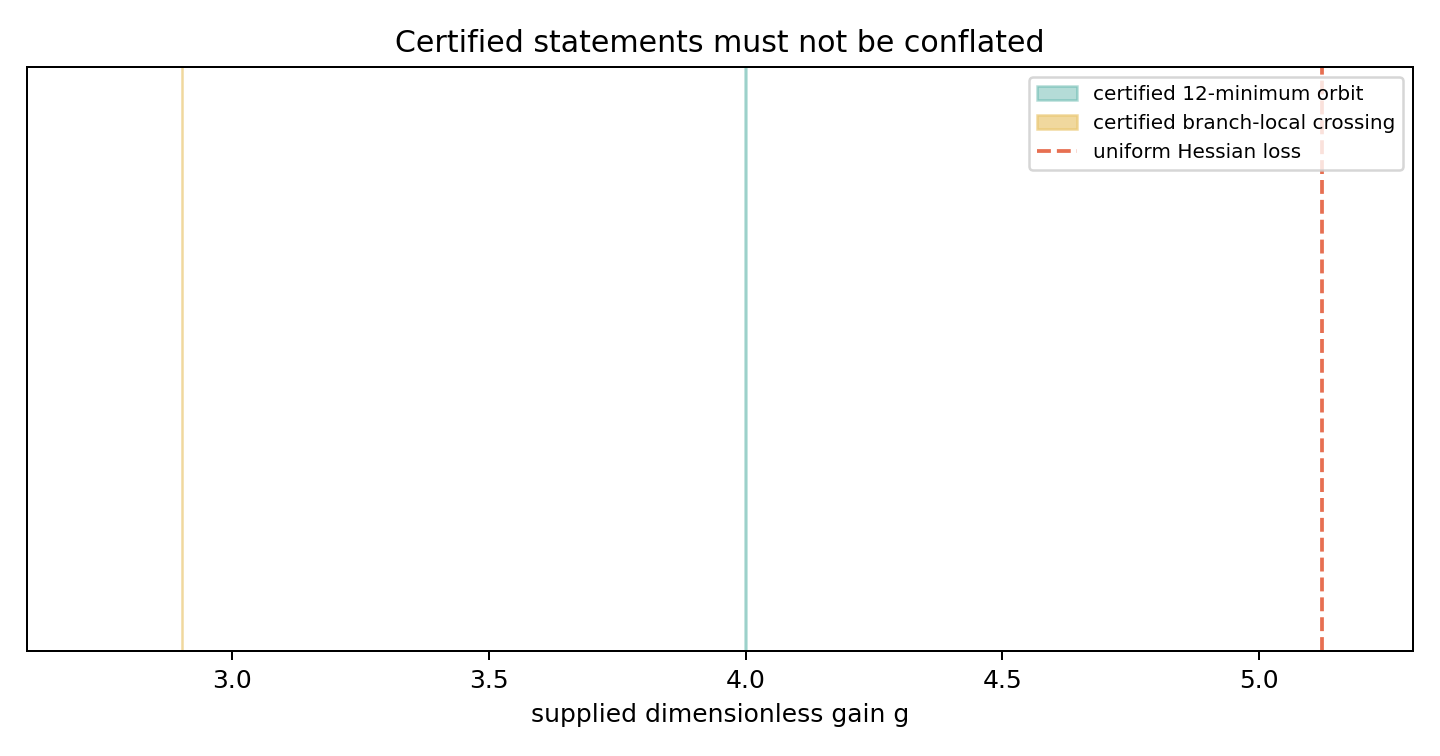
\includegraphics[width=.82\textwidth]{FIN_ST402_ST416_Figures/st405_gain_status.png}
\caption{Three different statements: branch coexistence, certified global persistence, and uniform Hessian loss.}
\end{figure}

\subsection{Morse landscape and local flow}

The uniform stationary point is an exact local minimum at $g=4$, with minimum
tangent Hessian eigenvalue $2.63127\ldots$.  The twelve localized global minima have
Morse index zero by the cap certificate.  In addition, 1,200 deterministic starts
found nine distinct $D_{12}$ stationary orbits: two numerical index-zero orbits,
four index-one orbits, and three index-two orbits.  Only the uniform and localized
minimum orbits are certified.  The saddle catalog is not an interval exhaustion.

\begin{figure}[H]
\centering
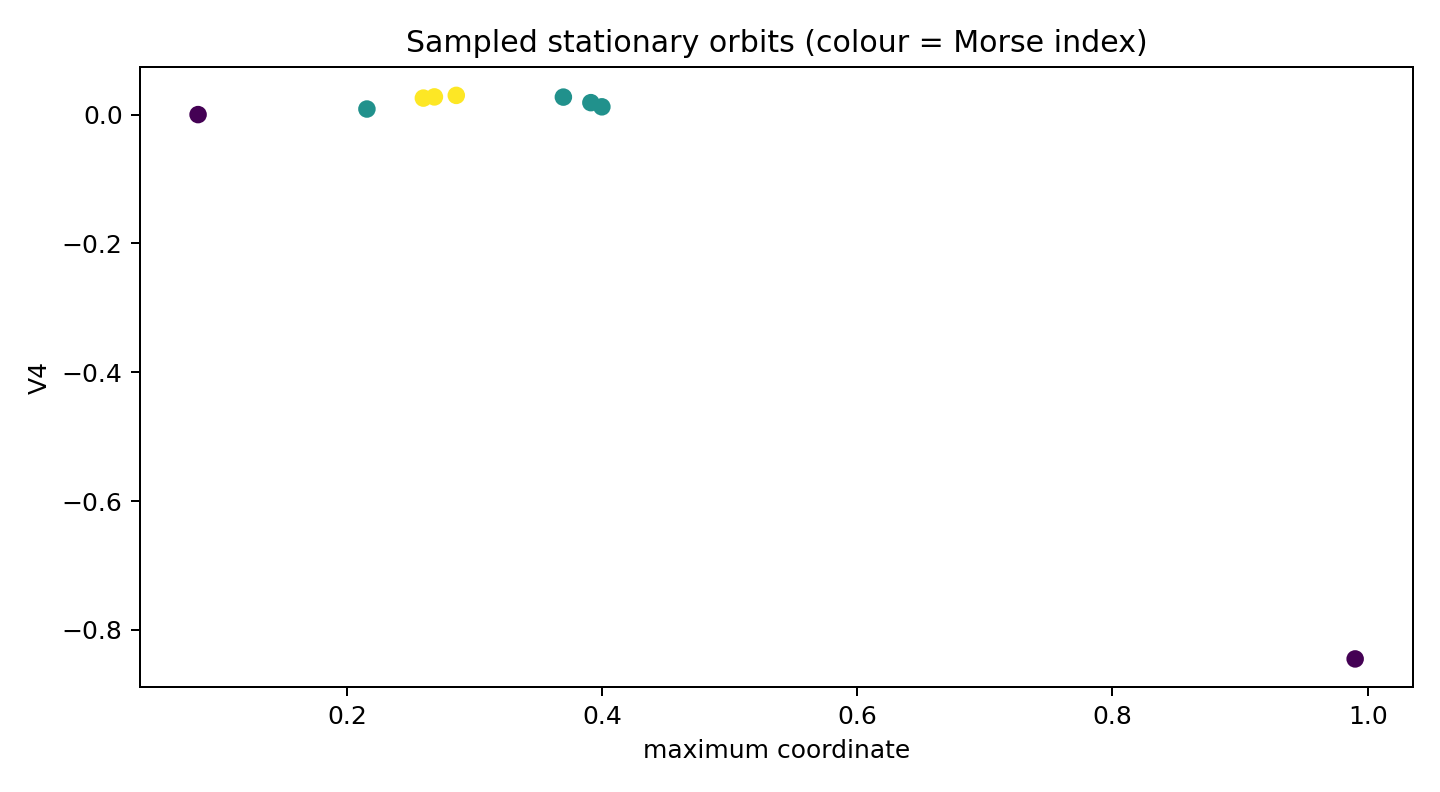
\includegraphics[width=.78\textwidth]{FIN_ST402_ST416_Figures/st407_morse_catalog.png}
\caption{Nonexhaustive sampled stationary-orbit catalog.  Colour encodes sampled Morse index.}
\end{figure}

For the explicitly supplied projected Euclidean flow
\[
 \dot p=-P_T\nabla V_4(p),\qquad P_T=I-\frac{\bm{1}\bm{1}^T}{12},
\]
the independent Krawczyk enclosure and cap curvature give a positive invariant ball
of radius $7.16\times10^{-5}$ around the cap-zero minimum.  Within this ball,
\[
 \lVert p(t)-p_*\rVert_2
 \le e^{-0.312161527688847t}\lVert p(0)-p_*\rVert_2.
\]
The flow, its time, preparation, and gain are premises.  This is neither a Born-rule
probability nor a physical relaxation rate.

\section{ST409--ST412: source stop, rank-seven obstruction, and invariants}

\subsection{Gain source and rank-seven nontransfer}

ST409 finds no new strict typed object that fixes the sign and magnitude of $g$ with
coupling semantics.  Deriving strong consequences from a supplied gain cannot be
reversed into a source theorem.

The rank-seven Fourier mediator also remains unresolved globally.  Its effective row
weights include four negative entries, with minimum $-0.17141297146\ldots$, so the
positive-weight water-filling theorem is inapplicable.  Its certified local root has
maximum probability about $0.903306$, below the approximately $0.93236$ threshold
at which the cap-curvature method becomes positive.  ST410 closes these two proof
routes only; it does not refute globality of the rank-seven state.

\subsection{First forced invariant relations}

The selected even $D_{12}$ invariant family contains six quadratic generators,
32 primitive quartic generators, and 117 primitive sextic generators.  Its formal
degree-eight products count as follows:
\[
 \binom{9}{4}=126,\qquad
 \binom{7}{2}32=672,\qquad
 \binom{33}{2}=528,\qquad
 6\cdot117=702.
\]
The total is 2,028.  Molien averaging gives dimension 1,892 for the complete
mean-zero degree-eight invariant space.  Therefore rank--nullity proves
\[
 \dim\ker(\text{degree-eight product map})\ge2028-1892=136.
\]
Because the declared degree-six candidate family had zero relations, degree eight
is the first forced relation degree in this chosen even generator construction.
An explicit minimal syzygy basis remains open.

\subsection{Algebraic versus statistical identifiability}

Exact modular work gives algebraic rank 365 for the sextic Reynolds basis under a
generic vertex-resolving evaluation design.  ST412 evaluates those 365 directions
at 500 frozen mean-zero unit vectors and normalizes every design column.  Numerical
rank remains 365, but
\[
 \sigma_{\min}=3.04179\times10^{-4},\qquad
 \kappa_2\approx1.50346\times10^4.
\]
For supplied observation noise $10^{-3}$, the worst least-squares coefficient
standard deviation is about $3.29$.  Thus exact distinguishability and stable noisy
recovery are not the same theorem.

\section{ST413: an adapted Chernoff cone}

The previous synthetic Chernoff transfer certificate used the coarse derivative
bound 6.6 and produced a gap near $2.5\times10^{-72}$.  For a binary emission
probability $q(b)=e_1+(e_0-e_1)b$ and Hilbert coordinate
$h=\log(b/(1-b))$, direct maximization gives
\[
 \max_b\left|\frac{d}{dh}\log q(b)\right|
 =\frac{|\sqrt{e_0}-\sqrt{e_1}|}{\sqrt{e_0}+\sqrt{e_1}}.
\]
For the frozen emissions this is at most $1/3$.  On
$s\in[0.45,0.55]$, the adapted product-metric weight Lipschitz constant is therefore
$11/60$, not 6.6.  With filter contraction $5/7$, the invariant cone slope becomes
$77/120$.  The resulting projective-diameter bound is $9.19769861$, and Birkhoff's
formula yields
\[
 1-\tanh(9.19769861/4)\ge0.0199262915891.
\]
This improves the explicit bound by 69.90 decimal orders.  The earlier microscopic
gap was principally a metric/bounding artefact, not evidence of intrinsically slow
mixing.  The entire result remains conditional on the synthetic HMM fixture.

\begin{figure}[H]
\centering
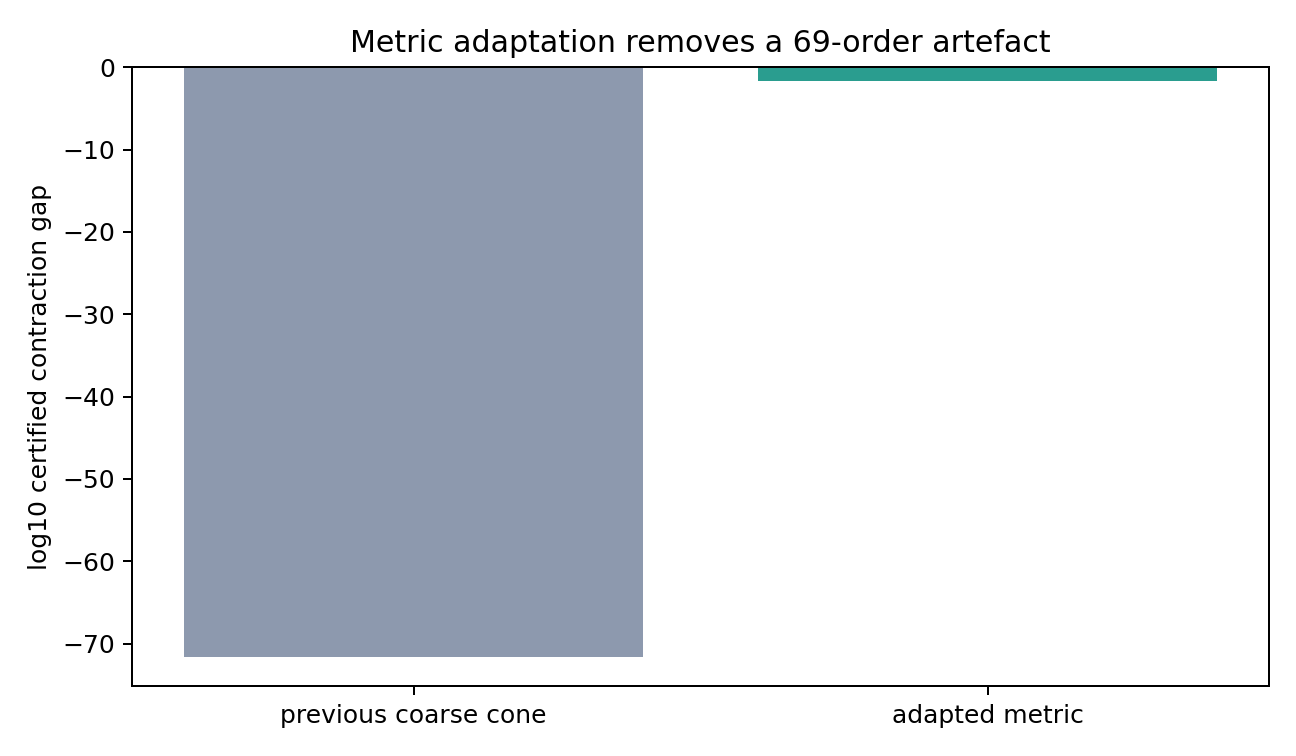
\includegraphics[width=.72\textwidth]{FIN_ST402_ST416_Figures/st413_gap_improvement.png}
\caption{The adapted Hilbert-coordinate calculation removes the coarse-cone artefact.}
\end{figure}

\section{ST414--ST415: expanded IR tube and a limiting band-loss face}

\subsection{A 55-fold wider root tube}

The supplied continuum-IR KKT system has central root
\[
 (y_1,y_2,y_3,a,\nu)=(0.0281902,2.1000678,2.5590976,0.0207319,0.1077760)\ldots .
\]
One common outward Krawczyk box now proves a unique root for every
\[
 B\in[2.9945,3.0055],\qquad T\in[3.9945,4.0055],
\]
using coordinate radii $(0.00055,0.022,0.0275,0.00055,0.0022)$.
The minimum inclusion margin is $8.94\times10^{-5}$.  This enlarges the ST395
parameter halfwidth by a factor 55.  A fixed-template bisection accepts through
$\delta=0.00554468$ and first fails at $0.00554492$; this brackets the limitation of
that one box template, not the maximal mathematical continuation domain.  The full
complement-sign topology cover was not re-certified on this enlarged rectangle.

\subsection{The compactified upper-band-loss face}

Numerical continuation toward smaller $T$ shows $a\downarrow0$ and
$y_3\uparrow\infty$.  Setting $a=0$ and compactifying $y_3=\infty$ leaves four
equations for $(y_1,y_2,\nu,T)$.  A fresh four-dimensional Krawczyk calculation
isolates their unique root in a radius-$10^{-8}$ box around
\[
 (0.028635829467935,\;3.89120890375954,\;0.0694500828220804,\;2.44218197709456).
\]
The inclusion margin is $9.9974\times10^{-9}$.

At this face the large-$y$ linear term disappears.  The third threshold escapes to
infinity and the upper active band vanishes.  What is proved is uniqueness of the
compactified limiting-face root.  The claim that the finite two-band branch attaches
to it is supported by residual-controlled continuation, but not by an interval
certificate for the singular attachment.

\begin{figure}[H]
\centering
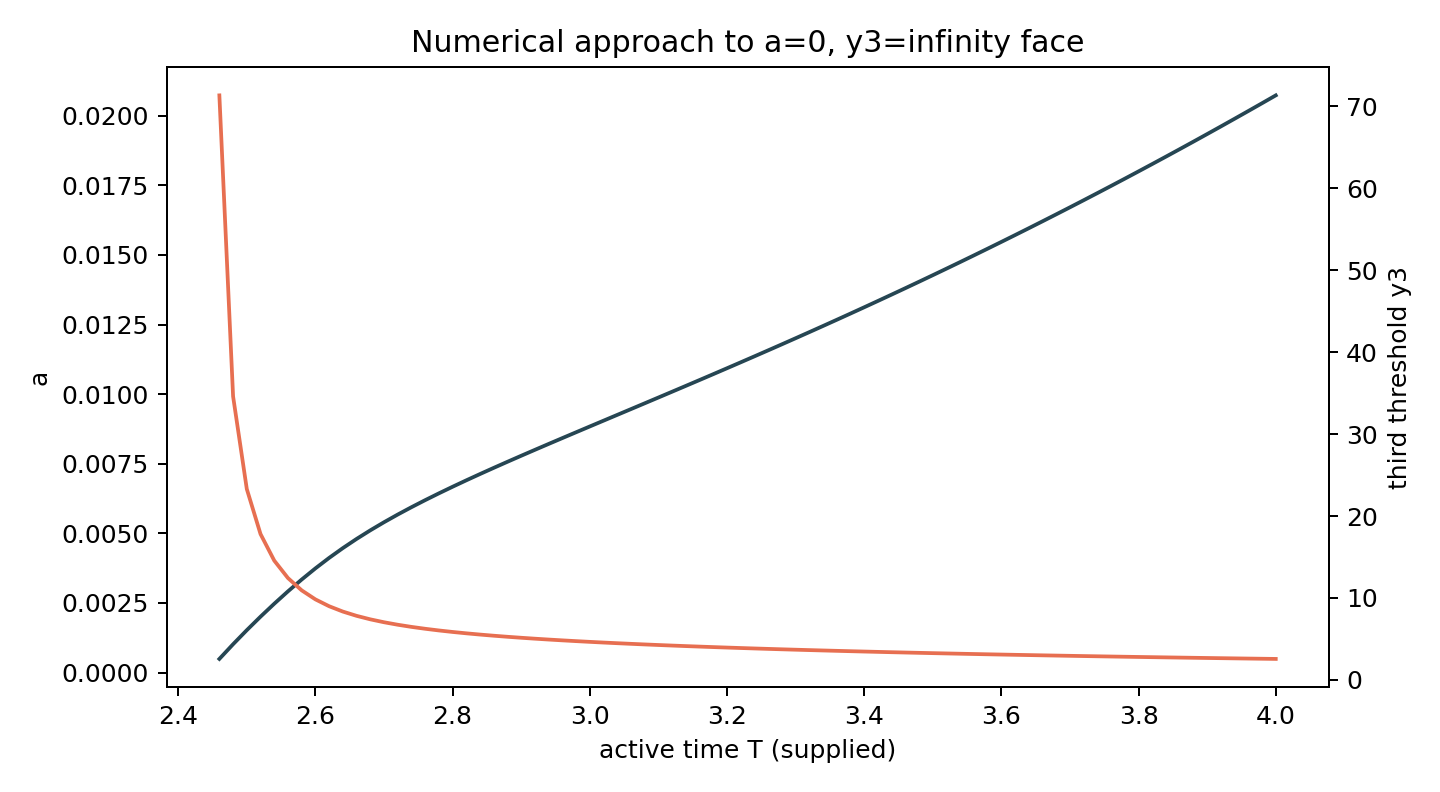
\includegraphics[width=.8\textwidth]{FIN_ST402_ST416_Figures/st415_band_loss.png}
\caption{Numerical approach to the interval-certified compactified face.  The displayed approach is evidence, not the face theorem itself.}
\end{figure}

\section{Falsification ledger and scientific interpretation}

The batch deliberately keeps negative outcomes visible.
\begin{itemize}[leftmargin=1.6em]
\item The exact orbit theorem does not select a realized vertex; it makes the
  selector obstruction sharper.
\item The gain tube proves robustness under a supplied coefficient but provides no
  source for that coefficient.
\item The branch-local crossing near $2.90249648$ is not promoted to a global
  transition.
\item The numerical Morse catalog is not an exhaustive stationary-point theorem.
\item The rank-seven global problem survives; two imported proof mechanisms fail.
\item Degree-eight rank--nullity proves a relation count lower bound, not explicit
  relations or a minimal presentation.
\item The Chernoff improvement concerns a synthetic fixture, not a detector.
\item ST414 certifies roots, not the full two-band topology on the enlarged box.
\item ST415 certifies a limiting face, not its singular branch attachment and not a
  physical phase boundary.
\end{itemize}

The deepest new mathematical interpretation is therefore precise but limited:
the supplied strict information functional has a robust, finite, symmetry-degenerate
landscape whose complete global minimum set is now independently certified.  It is
a theorem about consequences of symmetry and information geometry.  It is not yet
a theorem explaining why Nature supplies the functional, the gain, an orbit member,
or a dimensional realization.

\section{Recommended next programs ST417--ST431}

\begin{longtable}{>{\raggedright\arraybackslash}p{.08\textwidth}>{\raggedright\arraybackslash}p{.25\textwidth}>{\raggedright\arraybackslash}p{.55\textwidth}}
\toprule Priority&Program&Acceptance criterion\\\midrule\endhead
1&ST417 --- explicit degree-eight syzygy basis&Construct and exactly verify at least 136 independent relations; separate a basis from a mere dimension count.\\
1&ST418 --- global gain-transition enclosure&Combine gain-parametric cap/envelope proofs with certified competing branches; either isolate all global changes on a bounded range or report uncovered cells.\\
1&ST419 --- singular IR attachment theorem&Blow up $a\to0$, $y_3\to\infty$ and interval-certify attachment to the ST415 compactified face.\\
2&ST420 --- gain-tube enlargement&Optimize cap threshold and rational benchmarks to maximize the certified interval around $g=4$; report template versus theorem maximality.\\
2&ST421 --- stationary-orbit interval atlas&Certify the nine ST407 orbit candidates one by one and use a genuine global cover before claiming completeness.\\
2&ST422 --- Morse barrier graph&Once stationary orbits are certified, interval-bound heteroclinic barrier values and adjacency without assigning physical transition rates.\\
2&ST423 --- full enlarged IR topology cover&Restore complement-sign, inactive-slack, and tail certificates throughout the ST414 rectangle.\\
3&ST424 --- invariant-ring presentation&Compute generators and relations jointly through degree eight, including odd-degree sectors; stop under a declared resource budget.\\
3&ST425 --- optimal noisy invariant design&Choose evaluation states to maximize the smallest singular value under a frozen preparation/instrument class.\\
3&ST426 --- Chernoff gap sharpness&Compare the adapted cone bound with direct transfer-operator discretization and obtain certified upper and lower contraction brackets.\\
3&ST427 --- nonlinear local flow robustness&Add bounded perturbations to the declared projected flow and certify input-to-state stability of the local basin.\\
4&ST428 --- rank-seven sign-aware envelope&Develop an envelope that permits sign-changing effective weights; success requires a rigorous bound overlapping the local-root region.\\
4&ST429 --- source-admission theorem&Run only if a genuinely new strict typed object couples to $g$ with sign and magnitude; consequence-to-source inversion is forbidden.\\
5&ST430 --- selector/source theorem&Run only with a new non-premise symmetry-breaking provider; no replay of Aut$(\mathbb Z_{12})$-invariant selectors.\\
5&ST431 --- independent evidence gate&Require independently registered raw data or external audit; local code cannot satisfy this program.\\
\bottomrule
\end{longtable}

The preferred local order is ST417 $\to$ ST419 $\to$ ST418, with ST423 and
ST426 as independent secondary tracks.  ST429--ST431 are evidence/source gated and
must not be simulated by additional local algebra.

\section{Reproducibility}

The executable source is
\texttt{fin\_st402\_st416\_research.py}.  It writes one JSON packet per program,
the aggregate \texttt{FIN\_ST402\_ST416\_Results.json}, a CSV ledger, and four
figures.  The suite \texttt{test\_fin\_st402\_st416.py} contains 18 tests covering
matrix structure, independent interval inclusion, outside separation, curvature,
gain persistence, status boundaries, invariant counts, Chernoff constants, IR
certificates, and packet hashes.  All 18 tests pass in the recorded run.  A SHA-256
manifest accompanies the release.

The fixed random seed is 20260822.  The numerical stationary catalog and branch
continuation are explicitly separated from interval-certified statements.  Floating
solver success is nowhere used as a theorem of global exhaustion or phase change.

\begin{thebibliography}{9}
\bibitem{birkhoff} G. Birkhoff, ``Extensions of Jentzsch's theorem,''
\emph{Transactions of the American Mathematical Society} 85 (1957), 219--227.
\bibitem{cover} T. M. Cover and J. A. Thomas,
\emph{Elements of Information Theory}, 2nd ed., Wiley, 2006.
\bibitem{neumaier} A. Neumaier,
\emph{Interval Methods for Systems of Equations}, Cambridge University Press, 1990.
\bibitem{rockafellar} R. T. Rockafellar,
\emph{Convex Analysis}, Princeton University Press, 1970.
\bibitem{sturmfels} B. Sturmfels,
\emph{Algorithms in Invariant Theory}, 2nd ed., Springer, 2008.
\end{thebibliography}

\end{document}
